\chapter{Introduction}
This documentation contains information about the specifications, design, architecture and functionality of the dynamometer named Rolling Road. The system is designed with the goal of testing the performance of the electrically propulsed car 'AU2'.

It should be noted that the system is designed to work with 'AU2' and 'Rolling Road GUI'. These a threated as seperate systems and it is recommended that the reader reads their documentation, in order to get a complete overview the systems.

\begin{figure}[H]
	\centering
	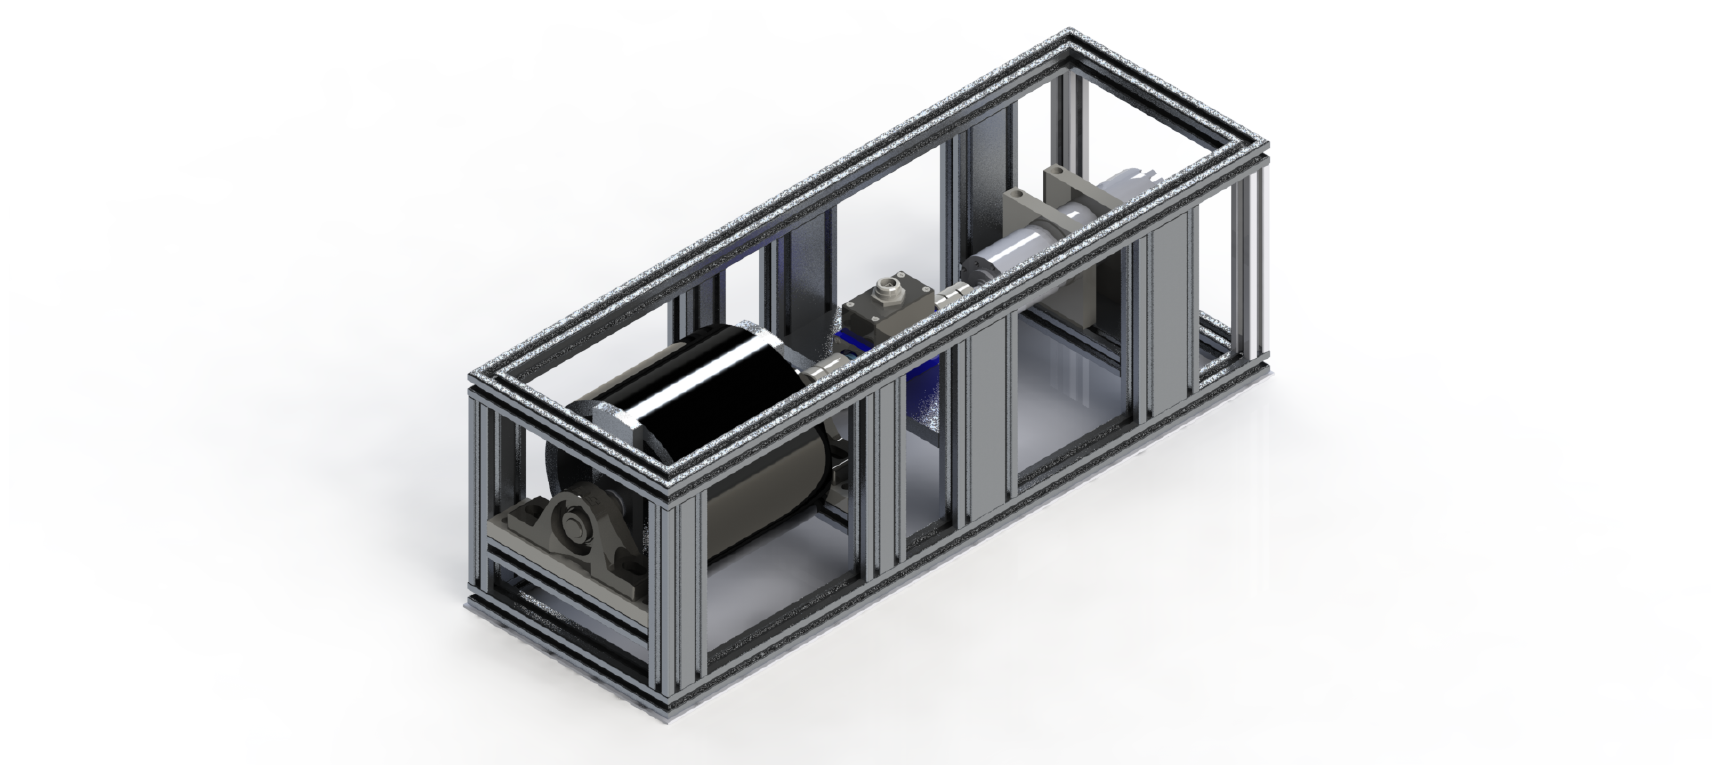
\includegraphics[width=0.5\linewidth]{Introduction/Model}
	\caption{Computer generated model of the system}
	\label{fig:System_model}
\end{figure}

\section{System description}
The primary purpose of the system is to measure the performance of an electrically propulsed car. The system has been designed with 'AU2' in mind but can also be used to test individual motors; as long as they meet the specifications.

The performance is tested in order to optimize the propulsion-algorithm in the car's motor controller. Testing is done by placing the car on top of the dynamometer and connecting the car's battery to the measurement-system. The performance is measured as the amount of electrical power from the battery which is directly converted to the mechanical energy which spins the car's wheel.

During the test the system will collect data from the test-drive and send them to the 'Rolling Road GUI' where they will be displayed graphically. The user is also able to regulate the amount of torque required to spin the roll in dynamometer, by using this GUI.

A quick overview of the system is shown in \ref{fig:System_overview}. It should be noted that neither the GUI nor 'AU2' are part of this system but are seperate systems which are required for complete functionality.

\begin{figure}[H]
	\centering
	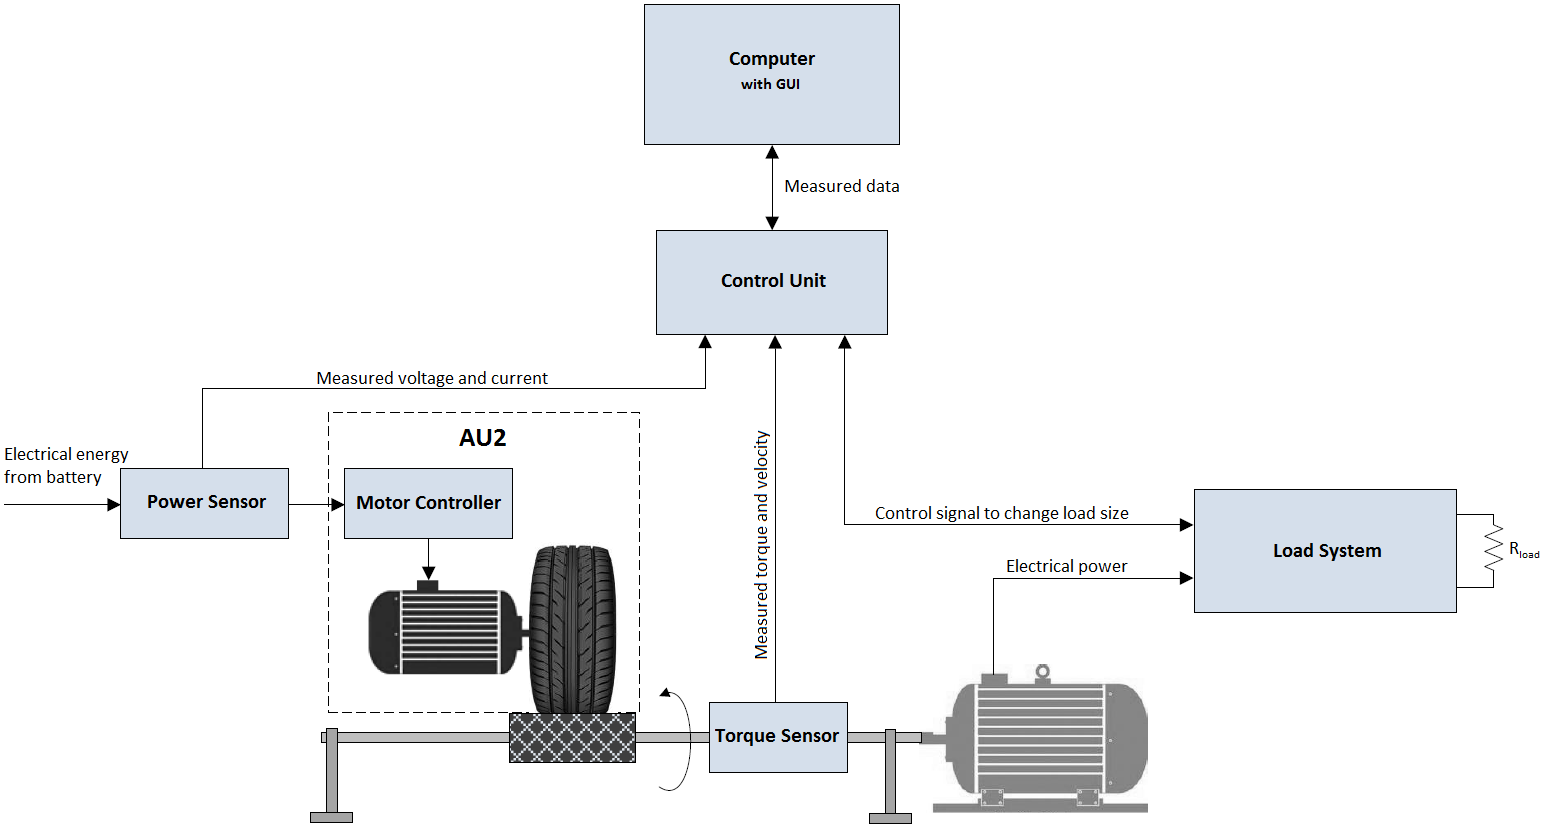
\includegraphics[width=1\linewidth]{Introduction/Overview}
	\caption{System overview}
	\label{fig:System_overview}
\end{figure}

\section{List of terms}
The following list explains the various terms which has been used to refer to certain parts or subsystems.
\begin{itemize}
	\item \textbf{Load}\\
	Refers to the amount of torque which is required to spin the roll in the dynamometer.
	\item \textbf{PSoC}\\
	Refers to the CY8CKIT-059 PSoC 5LP Prototype Kit which is used as the Control Unit in the system.
	\item \textbf{Something}\\
	Something else
\end{itemize}